\chapter{Methodology}
\label{sec:meth}

The usage of alert data with Machine Learning algorithms suffers from two issues; significant preprocessing must be performed to make the data have contextual meaning and methods to analyze the similarity of alerts are not well defined. For example, predicting a specific port which will be attacked only provides a small piece of significant data. However, a more significant feature to generate would be what type of service is typically run on a family of ports so that similar ports are grouped together. Additionally, when analyzing cyber alerts identifying the fidelity of data is not straight forward. In tasks such as event prediction results may be quantified by cross entropy loss on a per feature basis. But when generating new alerts there are complex interactions between various features which must be accounted for by the model. Simply generating \emph{a} realistic signature and port category is much less important than generating a realistic \emph{combination} of port signature and category. 

To address these challenges this section will cover the unique preprocessing applied to NIDS data collected from Suricata. Specifically, the features of alert signature, destination port, timestamp, and source IP will be considered. Additionally, intuitive metrics for analyzing alert fidelity are introduced as an inclusive system to address how realisitc generated alerts are compared to their source alerts from the ground truth dataset. 

\section{Network Intrusion Detection System Alerts Structure}

The structure of NIDS alerts can be seen graphically in Fig. \ref{fig:alert}. Note that this graphic does not display all the fields potentially in an alert. Some fields aren't always filled out. Some fields are deterministic from our experiements. 

\begin{figure}
	\centering
	\label{fig:alert}
	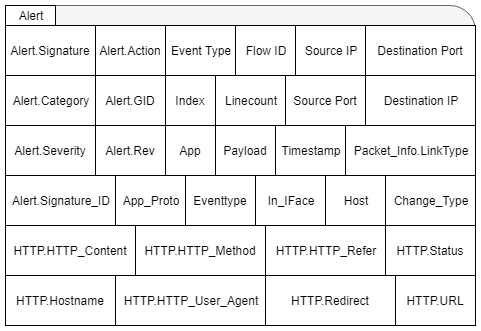
\includegraphics[width=\textwidth]{alert_struct}
	\caption{Sample Suricata Alert}
\end{figure}

\section{Cyber Alert Data Preprocessing}


The data used for these experiments comes from the National Collegiate Penetration Testing Competition from 2017 and 2018 (\texttt{https://nationalcptc.org/}). In 2017, teams were tasked with penetrating and exploiting network vulnerabilities in a virtualized network managing election systems. In 2018 teams were required to attack a multifaceted system handling autonomous cars which included host based systems, servers, and even mobile assets such as cell phones running an app. Each team had a total of 8 hours to scan, infiltrate, and exfiltrate information from the network. Both datasets provide a unique opportunity for Machine Learning experimentation as they are completely comprised of malicious actions as teams attempt to penetrate the target network. Though this data is unique to the competition it is worth noting that the preprocessing described herein is applicable to any dataset consisting of NIDS alerts.  

The first preprocessing step applied to the data was to separate alerts on a per-destination/target IP basis. This allowed individual models to be trained for each system on the network, typifying the type of traffic seen at that node. Additionally, data from all of the teams could be compounded, allowing for the number of potential attacks taken on a single target to be more fully expressed during training. Segmentation on a per-target basis has several intuitive benefits: First, it allows for different vulnerabilities to be highlighted on each machine given commonly occurring alert features at that target. Secondly, it helps to remove noisy alert influence from critical nodes in the network. For example, internet facing IPs may contain a significant amount of scanning activity, drowning out exfiltration related alert features at nodes further embedded in the network. Finally, the information extracted from alerts on a per target basis is actionable, as network administrators can use commonly targeted vulnerabilities to tune network settings for future defenses. 

% TODO: Numbers are for CPTC17 only -update with table

Next, the dimensionality of the destination port feature was reduced based off common service categories run across a collection of ports provided by the Internet Assigned Numbers Authority \cite{iana}. This reduction drops the number of unique values from 1516 destination ports to 69 destination port categories. Additionally, the dimensionality reduction step can easily be expanded or customized on a per network basis given a corporation's configuration of services. 

% TODO: Duplicate alerts are removed for 17, but not for 18. -retest


Finally, a set of simple statistical criterion are used to segment timestamps into bins. Traditional modeling of cyber attacks use killchain stages to segment actions into a series of contiguous stages with dependencies on previous stages. The beginning of an attack may consist of Reconnaissance based actions, yielding information about which IP to target in later attack stages. Similarly, the CPTC dataset may be segmented to try and capture unique behaviors into different bins of time. 

If applied to real world NIDS data another potential preprocessing step would be to segment source IPs based off of subnet. However, given that CPTC occurs in a virtualized network for a collegiate competition this preprocessing step is ignored. 

Following the methodology shown by \cite{us} bins are generated by smoothing the histogram timestamps and taking the first derivative to identify local minima and maxima. Then stages are cut if they contain at least $10\%$ of the total data and consecutive events at the candidate point contain less than $0.5\%$ of the total data. The goal of this ruleset is to capture significantly different types of traffic that does not split bursts of data into multiple stages.

\section{GAN Models}
\label{sec:model_arch}
Two GAN implementations were created to generate artificial cyber alert data; a standard Wasserstein GAN with Gradient Penalty and an extension of this model which used a neural estimate of mutual information to regularize the generator output.  

\subsection{Wasserstein GAN with Gradient Penalty}
\label{sec:gan}
The Wasserstein GAN with Gradient Penalty makes no architectural changes to model structure compared to standard GANs. Rather, the loss function is modified to use the Earthmover Distance. This modification has been shown to create empirically better results and allows for flexibility in model selection adapted to the challenge at hand.

Since the goal of this work was to create individual NIDS alerts without temporal correlation a feed-forward network architecture was selected for both the generator and discriminator. 

The generator consisted of 2 layers. The first layer sampled from noise space $\mathbb{Z}$ to a hidden representation. The next layer was directly responsible for each feature's output value. This layer consisted of four individual mappings from the hidden representation to an output layer with cardinality equal to the number of unique values per feature. Finally, a concatenation was used to take the prior 4 outputs and create a full 1-hot encoded alert. 

The discriminator also consisted of 2 layers. The first layer took 1-hot encoded alerts as input and mapped them to a hidden representation. The next layer mapped this hidden representation to a scalar value representing the probability that the alert was from the ground truth dataset. A graphical model is included in Fig. \ref{fig:model_simple}. Inputs to the network are highlighted in yellow. Learnable weight layers are in blue. The concatenation in orange is a non-backpropable layer used only to prepare generator output for input to the discriminator. The red boxes and lines represent the model loss functions and back-propagation.

\begin{figure}[!htbp]
	\centering%
	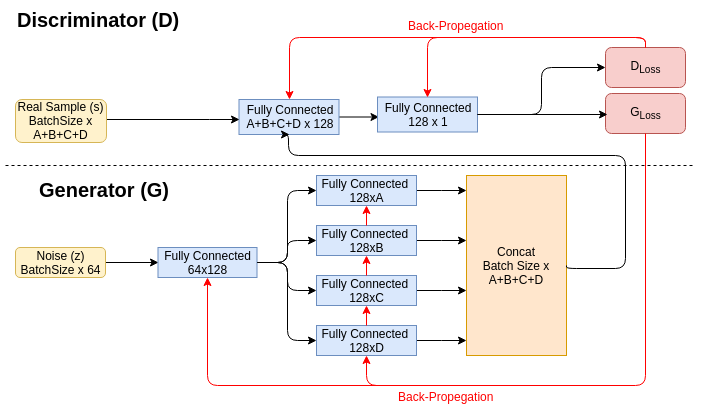
\includegraphics[width=\textwidth]{model_simple}
	\caption{WGAN-GP Model}
	\label{fig:model_simple}
\end{figure}

Table \ref{tab:model_simple_a} and Table \ref{tab:model_simple_b}, shows the dimensions of the weight matrices and activation functions for each layer of the network.


\begin{table}[!htbp]
	\centering
	\caption{Generator Network Architecture: Note that a-d are variable depending on the number of unique outputs}
	\label{tab:model_simple_a}
	\begin{tabular}{l|l|l}
		\hline
		\multicolumn{3}{c}{\textbf{Generator}} \\ 
		\hline
		\multicolumn{1}{c|}{Layer} & \multicolumn{1}{c|}{Matrix Dimensions} & \multicolumn{1}{c}{Activation Function} \\ \hline
		Input & 64 x 128 & ReLu \\
		Output - Feature 0 & 128 x a & NA \\
		Output - Feature 1 & 128 x b & NA \\
		Output - Feature 2 & 128 x c & NA \\
		Output  - Feature 3 & 128 x d & NA \\
		Concatenation & a+b+c+d & NA \\
		\hline
	\end{tabular}
\end{table}

\begin{table}[!htbp]
	\centering
	\caption{Discriminator Network Architecture: Note that a-d are variable depending on the number of unique outputs}
	\label{tab:model_simple_b}
	\begin{tabular}{l|l|l}
		\hline
		\multicolumn{3}{c}{\textbf{Discriminator}} \\ 
		\hline
		\multicolumn{1}{c|}{Layer} & \multicolumn{1}{c|}{Matrix Dimensions} & \multicolumn{1}{c}{Activation Function} \\ \hline
		Input & a+b+c+d x 128 & ReLu \\
		Output & 128 x 1 & Sigmoid \\
		\hline
	\end{tabular}
\end{table}


\subsection{Mutual Information Neural Estimator}
\label{sec:mine}
Mutual Information is a measure of dependence between two random variables. Traditionally, approximations have to be used to estimate the mutual information between high dimensional and continuous variables as exact computation is intractable. The Mutual Information Neural Estimator is a neural network which allows for state of the art approximation of mutual information. This is done by optimizing the network to minimize the Donsker-Varadhan representation of the KL divergence between two variables. 

A feed forward neural network was implemented to learn the mutual information between the gaussian noise sampled from $\mathbb{Z}$ and the generators output. This network consisted of 2 layers. The first layer took input from each of the aforementioned sources and mapped them to separate hidden representation layers and added together. Then the second layer mapped the hidden representation to a single output value representing the mutual information estimate. Table \ref{tab:model_mi} shows the matrix dimension for each of the layers in the network.

\begin{table}[!htbp]
	\centering
	\caption{Mutual Information Estimator Network Architecture: Note that a-d are variable depending on the number of unique outputs}
	\label{tab:model_mi}
	\begin{tabular}{l|l|l}
		\hline
		\multicolumn{3}{c}{\textbf{Estimator}} \\ 
		\hline
		\multicolumn{1}{c|}{Layer} & \multicolumn{1}{c|}{Matrix Dimensions} & \multicolumn{1}{c}{Activation Function} \\ \hline
		Input - Generated & a+b+c+d x 128 & ReLu \\
		Input - Noise & 64 x 128 & NA \\
		Addition & 128 & NA \\ 
		Output & 128 x 1 &  NA \\
		\hline
	\end{tabular}
\end{table}


\subsection{WGAN-GP with Mutual Information Constraint}
\label{sec:gpmi}

In order to improve mode dropping in the GAN model described in Section \ref{sec:gan} the mutual information neural estimator in Section \ref{sec:mine} is added to the model. This is done by using the mutual information between the generated samples and the input noise as a proxy for the neg-entropy of the samples and using it to regularize the generator's weights. We refer to this model as the Wasserstein GAN with Gradient Penalty and Mutual Information (WGAN-GPMI). Fig. \ref{fig:model_complex} shows what the full model consists of. The addition of the Mutual Information Estimation Network helps to enforce that the generator must learn all output modes of the distribution by fully exploiting the noise sample

\begin{figure}[!htbp]
	\centering%
	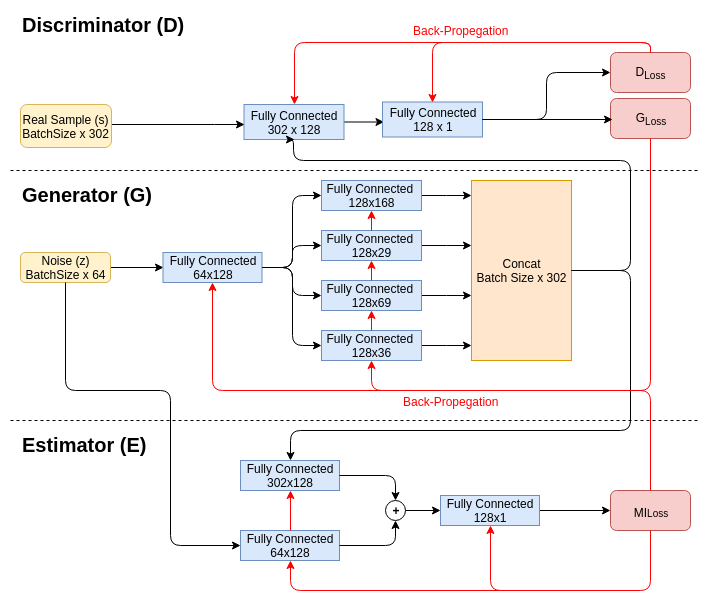
\includegraphics[width=\textwidth]{model_complex}
	\caption{WGAN-GPMI Model}
	\label{fig:model_complex}
\end{figure}

Since mutual information is theoretically unbounded, gradient updates resulting from it could overwhelm the adversarial gradients resulting from the Earthmover Distance. In order to address this all of the gradient updates to the generator are adaptively clipped to ensure that the Frobenius norm of the gradient resulting from the mutual information is at most equal to the adversarial gradient \cite{Belghazi2018}.


\subsection{Model Training}
\label{sec:training}

Training GANs is a notoriously tricky task as loss score is not a fair representation of whether the model has converged to generating realistic data. Like many traditional Deep Learning models, hyperparameter tuning is critical to model performance for GANs. This creates a challenge while training GANs, especially with unconventional datasets where metrics like Inception Score cannot be applied. In order to address this and exhaustive hyperparameter search for each of the GAN models above was carried out. First, individual parameters were tuned in order to find candidate values. Then, these candidate values were used in a search of all possible parameter combinations.

Using the histogram intersection metric proposed in Section \ref{sec:anal} across all combinations of features, the hyperparameter setting which achieved the most intersection scores in the $90^{th}$ percentile were selected as optimal. More details about the result of this search will be covered in Section \ref{sec:rna}.